\chapter{Test of type area}
\label{chap:typeareatest}

Far far away, behind the word mountains, far from the countries Vokalia and Consonantia, there live the blind texts. Separated they live in Bookmarksgrove right at the coast of the Semantics, a large language ocean. A small river named Duden flows by their place and supplies it with the necessary regelialia. It is a paradisematic country, in which roasted parts of sentences fly into your mouth. Even the all-powerful Pointing has no control about the blind texts it is an almost unorthographic life One day however a small line of blind text by the name of Lorem Ipsum decided to leave for the far World of Grammar. 

\section{The Big Oxmox}
\label{sec:typeareatest_ombox}

The Big Oxmox advised her not to do so, because there were thousands of bad Commas, wild Question Marks and devious Semikoli, but the Little Blind Text didn’t listen. She packed her seven versalia, put her initial into the belt and made herself on the way. When she reached the first hills of the Italic Mountains, she had a last view back on the skyline of her hometown Bookmarksgrove, the headline of Alphabet Village and the subline of her own road, the Line Lane. Pityful a rethoric question ran over her cheek, then she continued her way. On her way she met a copy.

\begin{equation}
	\mathcal{N}(x \mid \mathbold{\mu}, \mathbold{\Sigma}) = \frac{1}{(2\pi)^{D/2}} \frac{1}{|\mathbold{\Sigma}|^{(1/2)}} \exp \left( -\frac{1}{2}(x-\mathbold{\mu})^{T}\mathbold{\Sigma}^{-1}(x-\mathbold{\mu}) \right)
\end{equation}

The copy warned the Little Blind Text, that where it came from it would have been rewritten a thousand times and everything that was left from its origin would be the word "and" and the Little Blind Text should turn around and return to its own, safe country. But nothing the copy said could convince her and so it didn’t take long until a few insidious Copy Writers ambushed her, made her drunk with Longe and Parole and dragged her into their agency, where they abused her for their projects again and again. And if she hasn’t been rewritten, then they are still using her.

\section{Type dummy text}
\label{sec:typeareatest_typedummytext}

This is a typo dummy text. On it you can see if all the letters there are and how they look. Sometimes one uses words like Hamburgefonts, Rafgenduks or Handgloves to test fonts. Sometimes phrases that contain all letters of the alphabet - one calls these sets "pangrams".

Well known is this: The quick brown fox jumps over the lazy old dog. Often in type dummy texts also foreign-language sentence parts are installed (AVAIL\textsuperscript{\texttrademark} and Wefox\textsuperscript{\textregistered} are testing aussi la Kerning) to test the effect in other languages. In Latin, for example, almost every font looks good.

\subsection{Demonstrandum}
\label{subsec:satzspiegeltest_typoblindtext_demonstrandum}

Quod erat demonstrandum. Seit 1975 fehlen in den meisten Testtexten die Zahlen, weswegen nach TypoGb. 204 \S ab dem Jahr 2034 Zahlen in 86 der Texte zur Pflicht werden. Nichteinhaltung wird mit bis zu 245 \texteuro oder 368\$ bestraft. Genauso wichtig in sind mittlerweile auch \^A\c{c}c\`e\~nt\"e, die in neueren Schriften aber fast immer enthalten sind. Ein wichtiges aber schwierig zu integrierendes Feld sind OpenType-Funktionalit\"aten. Je nach Software und Voreinstellungen k\"onnen eingebaute Kapit\"alchen, Kerning oder Ligaturen (sehr pfiffig) nicht richtig dargestellt werden.

\subsubsection{Subsubsection}

This is a typo dummy text. On it you can see if all the letters there are and how they look. Sometimes one uses words like Hamburgefonts, Rafgenduks or Handgloves to test fonts. Sometimes phrases that contain all letters of the alphabet - one calls these sets "pangrams". 

\subsubsection{Subsubsection}

Well known is this: The quick brown fox jumps over the lazy old dog. Often in type dummy texts also foreign-language sentence parts are installed (AVAIL\textsuperscript{\texttrademark} and Wefox\textsuperscript{\textregistered} are testing aussi la Kerning) to test the effect in other languages. In Latin, for example, almost every font looks good. Quod erat demonstrandum.

\section{Webstandards}
\label{sec:satzspiegeltest_webstandards}

Everywhere the same old story. The layout is complete, the text is slow in coming. This layout is now not naked in space and small and empty occurs, I help out: the dummy text. Created exactly for this purpose, always in the shadow of my big brother "Lorem Ipsum", I look forward every time you read a few lines. Because esse est percipi - being is to be perceived.

And now because you already have the goodness to accompany me a few more sentences long, I would like to take this opportunity to serve you not only as a stopgap, but to point out something that is going to be perceived as deserved: Web viz. See Web standards are the rules that build on the websites. So there are rules for HTML, CSS, JavaScript or XML, words that you might have heard of your developers. These standards ensure that all parties the maximum benefit from a website.

\begin{figure}[H]
	\centering
		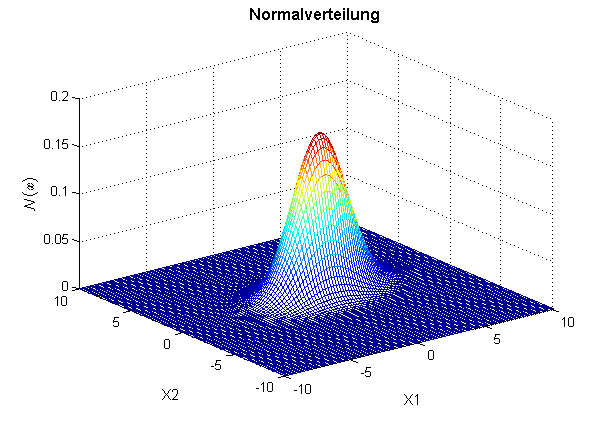
\includegraphics[scale=0.7]{images/multivariate_gauss.png}
	\caption{Normal distribution}
	\label{fig:normal_distribution}
\end{figure}

In contrast to previous websites we no longer need, for example, two different sites for the program Internet Explorer and another browser. It extends a page that - properly applied - both works on different browsers on the net, but just as good for printing or display on a cell phone is. Mind: A site for all formats. What a relief. Standards save time provide for the development costs and ensure that web pages can be easier to maintain later. Of course, only if everyone adheres to these standards.
